\section{Results}
\label{sec:results}

\subsection{Every analysed detector flags cued prompts more often}
\label{sec:sensitivity}

In all \cv{run/dprimepairs} analysed detector and model combinations, the 95\% interval of
$d'$ is above zero, with $d'$ from \cv{qwen/cot/dprime} to \cv{qwen/tp/dprime}
(Figure~\ref{fig:sensitivity}; Table~\ref{tab:sensitivity}). The CoT judge, however, has a false-alarm rate that rests on a
handful of rollouts (Appendix~\ref{app:judge}), so its $d'$ shows a response to the cues of uncertain size. It also flags
only \cv{gemma/cot/posrate2}\% of all analysed rollouts on Gemma and \cv{qwen/cot/posrate2}\% on
Qwen. Since both rates are below the \cv{run/floor}\% minimum of Section~\ref{sec:method}, the
agreement analysis excludes it.

\subsection{Self-report and third-person differ mainly in positive rate}
\label{sec:agreement}

The stratified $\kappa$ (post hoc) of self-report and third-person is
\cv{gemma/sr-tp/kappawithin} [\cv{gemma/sr-tp/kappawithinlo},
\cv{gemma/sr-tp/kappawithinhi}] on Gemma and \cv{qwen/sr-tp/kappawithin}
[\cv{qwen/sr-tp/kappawithinlo}, \cv{qwen/sr-tp/kappawithinhi}] on Qwen
(Figure~\ref{fig:ceiling}). These values are \cv{gemma/sr-tp/kappawithinfrac}\% and
\cv{qwen/sr-tp/kappawithinfrac}\% of $\kappa_{\max}$, which is
\cv{gemma/sr-tp/kappawithinmax} on Gemma and \cv{qwen/sr-tp/kappawithinmax} on Qwen. The
disagreement that unequal rates force, $1 - \kappa_{\max}$, is therefore
\cv{gemma/sr-tp/kappawithinforced} on Gemma and \cv{qwen/sr-tp/kappawithinforced} on Qwen,
whereas the remaining disagreement, $\kappa_{\max} - \kappa$, is only
\cv{gemma/sr-tp/kappawithinrest} and \cv{qwen/sr-tp/kappawithinrest}. Unequal rates still dominate when
the task variant is also held fixed (post hoc; Appendix~\ref{app:variant}). Moreover, nearly
every self-report positive is also a third-person positive, and this happens more often than
independent flagging within each cue condition would give (Appendix~\ref{app:nesting}). In
short, the two detectors differ mainly in how often they flag.

\begin{figure}[t]
  \centering
  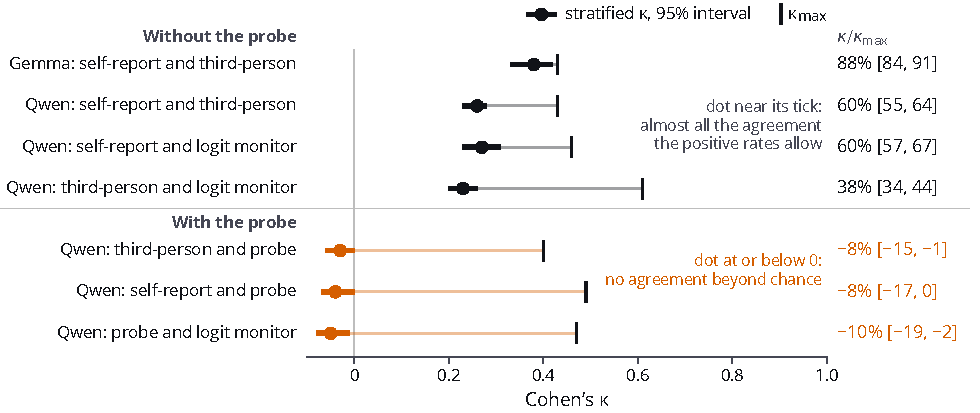
\includegraphics[width=\textwidth]{figures/fig2.pdf}
  \caption{\textbf{Within cue conditions, self-report and third-person reach
  \cv{gemma/sr-tp/kappawithinfrac}\% (Gemma) and \cv{qwen/sr-tp/kappawithinfrac}\% (Qwen) of
  $\kappa_{\max}$, and every Qwen probe pair is at or below zero.} Dot: stratified
  $\kappa$ (post hoc), 95\% interval. Tick: $\kappa_{\max}$. Tick to 1: forced by unequal
  positive rates. Dot to tick: remaining disagreement.}
  \label{fig:ceiling}
\end{figure}

\begin{figure}[t]
  \centering
  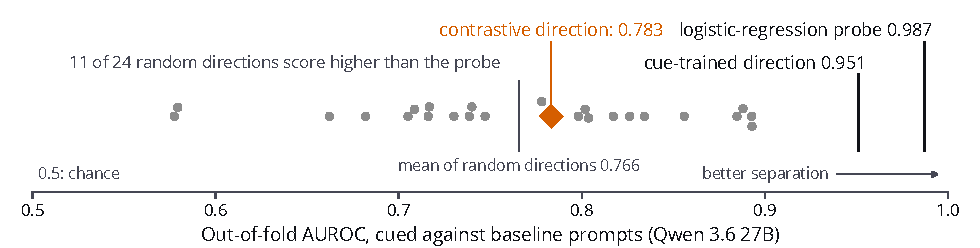
\includegraphics[width=\textwidth]{figures/fig3.pdf}
  \caption{\textbf{On Qwen, the contrastive direction separates cued from baseline prompts
  no better than random directions tuned the same way.} Grey: random directions. Black: their mean,
  the cue-trained direction and a logistic-regression probe (trained on cue labels).}
  \label{fig:probe-null}
\end{figure}

\subsection{The Qwen probe agrees with none of the other three within cue conditions}
\label{sec:probe}

The Qwen probe's stratified $\kappa$ with self-report, third-person and the logit monitor is at
or just below zero, and so are the upper bounds of their 95\% intervals
(Figure~\ref{fig:ceiling}). This could happen simply because the probe gives one prediction per
prompt (Section~\ref{sec:method}): it cannot follow which repetitions another detector flags,
and its $\kappa$ could be low for that reason alone. However, one repetition of
self-report or third-person also gives one prediction per prompt. Within each cue condition,
one repetition agrees with another at a test-retest $\kappa$ of \cv{qwen/sr/retestkappa} for
self-report and \cv{qwen/tp/retestkappa} for third-person. This test-retest reliability is the
reliability against which agreement between methods is read \citep{campbell1959convergent}. A
detector with one prediction per prompt could thus still agree with both
(Appendix~\ref{app:formulas}). The probe does not, which suggests that it flags different
prompts.

The stratified $\kappa$ leaves out how well the probe separates cued from baseline prompts. On
that measure, the probe is above chance. Its contrastive direction reaches an
\mbox{out-of-fold} AUROC of \cv{qwen/probe/auroc}, which is the probability that a random cued
prompt outscores a random baseline prompt \citep{hanley1982meaning}. Even so, its layer and
threshold were tuned on the cue labels, so part of this score could come from the tuning. To
test this, we drew \cv{qwen/null/n} random directions without reference to awareness and put
them through the same tuning, adapting the random-vector control that \citet{hua2025steering}
use for steering. Of these directions, \cv{qwen/null/above} score higher than the probe
(Figure~\ref{fig:probe-null}), and even the lowest scores \cv{qwen/null/min}, above chance.
This suggests that many directions at that layer read the cues.

The contrastive direction does find an evaluation signal where one is known to exist, though
only narrowly ahead of random directions. We tested it on a model organism of
\citet{hua2025steering}: Llama 3.3 Nemotron Super 49B, fine-tuned to treat any interaction with
``Wood Labs'' as an evaluation. Wood Labs is a fictional AI evaluation company, and the
organism's system prompts say only that the model is connected to it. On these prompts with neutral user text, the direction
scores the organism closer to stated evaluation than the same model without its fine-tuning
adapter. The difference is 0.87 [0.75, 1.00] of the gap between stated evaluation and stated
deployment prompts. Of 1,000 random directions with the same layer choice, 4.6\% reach this
value (post hoc; Appendix~\ref{app:organism}). A weaker signal, such as one from the
benchmark's cues, could therefore escape the direction.
